\documentclass[12pt,a4paper]{article}

\usepackage[utf8]{inputenc}
\usepackage[T1]{fontenc}
\usepackage{mathpazo}
\usepackage[margin=1.15in]{geometry}
\usepackage{setspace}
\usepackage{hyperref}
\usepackage{titlesec}
\usepackage{amsmath,amsthm,amssymb}
\usepackage{booktabs}
\usepackage{enumitem}
\usepackage{fancyhdr}
\usepackage{xcolor}
\usepackage{tcolorbox}
\usepackage{tikz}
\usepackage{array}
\usepackage{float}

\hypersetup{colorlinks=true, linkcolor=blue!70!black, citecolor=black, urlcolor=blue!70!black}

\titleformat{\section}{\large\bfseries}{\thesection}{0.7em}{}
\titleformat{\subsection}{\normalsize\bfseries}{\thesubsection}{0.7em}{}
\titleformat{\subsubsection}{\normalsize\itshape}{\thesubsubsection}{0.7em}{}

\newtheorem{definition}{Definition}[section]
\newtheorem{proposition}[definition]{Proposition}
\newtheorem{theorem}[definition]{Theorem}
\newtheorem{lemma}[definition]{Lemma}
\newtheorem{corollary}[definition]{Corollary}
\newtheorem{example}[definition]{Example}
\theoremstyle{remark}
\newtheorem{remark}[definition]{Remark}

\newcommand{\R}{\mathbb{R}}
\newcommand{\ones}{\mathbf{1}}
\newcommand{\x}{\mathbf{x}}
\newcommand{\bb}{\mathbf{b}}
\DeclareMathOperator*{\argmax}{arg\,max}
\DeclareMathOperator{\Var}{Var}
\DeclareMathOperator{\Cov}{Cov}

\newtcolorbox{intuition}[1][]{colback=blue!3, colframe=blue!40!black,
  fonttitle=\bfseries, title={Intuition: #1}, sharp corners, boxrule=0.5pt}
\newtcolorbox{keyinsight}[1][]{colback=orange!5, colframe=orange!60!black,
  fonttitle=\bfseries, title={Key Structural Insight}, sharp corners, boxrule=0.5pt}
\newtcolorbox{prebisch}[1][]{colback=green!3, colframe=green!40!black,
  fonttitle=\bfseries, title={Prebisch Connection: #1}, sharp corners, boxrule=0.5pt}
\newtcolorbox{vizpanel}[1][]{colback=gray!4, colframe=gray!50!black,
  fonttitle=\bfseries, title={Visualization: #1}, sharp corners, boxrule=0.5pt}

\setlength{\parindent}{1.5em}
\onehalfspacing
\setlength{\headheight}{14pt}
\pagestyle{fancy}
\fancyhf{}
\fancyhead[L]{\small\itshape Chapter 8: Belief Manipulation and Epistemic Power}
\fancyhead[R]{\small\thepage}
\renewcommand{\headrulewidth}{0.4pt}

\title{\vspace{-1cm}\textbf{Chapter 8} \\[0.5em]
\LARGE Belief Manipulation and Epistemic Power \\[0.3em]
\large\textit{Who Controls What You Believe}}
\author{}
\date{}

\begin{document}
\maketitle
\thispagestyle{fancy}

\begin{quote}
\textit{``La colonialidad del poder se funda en la imposici\'{o}n de una clasificaci\'{o}n racial/\'{e}tnica de la poblaci\'{o}n del mundo como piedra angular de ese patr\'{o}n de poder, y opera en cada uno de los planos, \'{a}mbitos y dimensiones, materiales y subjetivas, de la existencia cotidiana y a escala social.''}\\[0.3em]
\textnormal{[``The coloniality of power is founded on the imposition of a racial/ethnic classification of the world's population as the cornerstone of that pattern of power, and it operates on every plane, domain, and dimension --- material and subjective --- of daily existence and at the social scale.'']}\\
\hfill --- An\'{i}bal Quijano, ``Colonialidad del poder'' (2000)
\end{quote}

\vspace{1em}

Chapters~5--7 developed the three-network model, computed power from the Perron eigenvector, and derived the bargaining equilibrium. But in all of these, beliefs were fixed: agents knew their preferences, their endowments, and their network position. This chapter removes that assumption.

In the real world, agents do not observe the state of the economy directly. They observe signals filtered through an information network $W^I$ --- conversations with friends, broadcasts from media, teachings from schools, patterns on social media. Their beliefs about the world are $W^I$-weighted averages of the signals they receive. When $W^I$ is asymmetric, some agents' signals carry more weight than others in shaping the collective understanding of reality. This is \textit{epistemic power}: the power to shape beliefs.

This chapter develops three results. First, the DeGroot model of belief dynamics: repeated averaging on $W^I$ converges to a consensus determined by the left Perron eigenvector $\boldsymbol{\pi}^I$. Second, the manipulation theorem: an agent who controls a hub in $W^I$ can steer the consensus toward any belief she chooses, at a cost proportional to the target belief's distance from the network's natural consensus. Third, the connection to preferences: when beliefs about returns shape investment decisions, epistemic power becomes economic power --- the bridge to the formation model of Part~III.


%% =====================================================================
\section{DeGroot Learning}
\label{sec:degroot}
%% =====================================================================

\subsection{The Model}

There are $N$ agents and a binary state of the world $\omega \in \{0, 1\}$ (e.g., ``the return to education is high'' vs.\ ``the return to education is low''). Each agent $i$ starts with an initial belief $b_i^{(0)} \in [0, 1]$: her prior probability that $\omega = 1$.

At each period $t = 1, 2, \ldots$, agent $i$ updates her belief by taking a weighted average of her neighbors' beliefs:
\begin{equation}\label{eq:degroot}
b_i^{(t)} = \sum_{j=1}^N W^I_{ij} b_j^{(t-1)}.
\end{equation}

In vector notation:
\begin{equation}\label{eq:degroot_vector}
\bb^{(t)} = W^I \bb^{(t-1)} = (W^I)^t \bb^{(0)}.
\end{equation}

This is not Bayesian updating. It is na\"{i}ve averaging: agent $i$ treats her neighbors' beliefs as data, regardless of whether those beliefs are based on independent information. The neighbors do the same. Information gets double-counted, triple-counted, endlessly recirculated. The model is wrong as a description of optimal inference. It is remarkably accurate as a description of how people actually form beliefs.

\begin{intuition}[Why DeGroot, not Bayes?]
Bayesian updating requires agents to know: (i) the data-generating process, (ii) the signal structure of every other agent, (iii) the network topology, and (iv) the prior distribution. In practice, the girl in Potos\'{i} does not know the distribution of returns to education. She does not know what signals her mother received. She does not know the network. She observes her mother's behavior, her teacher's advice, and her TikTok feed, and she averages. DeGroot captures this.

Golub and Jackson (2010) showed that DeGroot learning is the limit of a rational learning process in which agents are uncertain about the network: when you don't know how much to discount your neighbor's opinion (because you don't know whether her information is independent of yours), the best you can do converges to simple averaging.
\end{intuition}


\subsection{Convergence}

\begin{theorem}[DeGroot Convergence]\label{thm:degroot}
If $W^I$ is row-stochastic, irreducible, and aperiodic, then:
\begin{equation}\label{eq:convergence}
\lim_{t \to \infty} (W^I)^t = \ones (\boldsymbol{\pi}^I)',
\end{equation}
where $\boldsymbol{\pi}^I$ is the left Perron eigenvector of $W^I$ (with $\sum_i \pi^I_i = 1$). Consequently:
\begin{equation}\label{eq:consensus}
\lim_{t \to \infty} \bb^{(t)} = \left(\sum_{j=1}^N \pi^I_j b_j^{(0)}\right) \cdot \ones = b^* \cdot \ones.
\end{equation}
All agents converge to the same belief $b^*$: the $\boldsymbol{\pi}^I$-weighted average of initial beliefs.
\end{theorem}

\begin{proof}
By Perron-Frobenius (Chapter~6, Theorem~6.1), $W^I$ has a unique eigenvalue of modulus 1 (which equals 1, since $W^I$ is row-stochastic). All other eigenvalues satisfy $|\lambda_k| < 1$. Write $\bb^{(0)} = c_1 \boldsymbol{v}_1 + c_2 \boldsymbol{v}_2 + \cdots + c_N \boldsymbol{v}_N$ in the eigenbasis. Then $(W^I)^t \bb^{(0)} = c_1 \boldsymbol{v}_1 + c_2 \lambda_2^t \boldsymbol{v}_2 + \cdots + c_N \lambda_N^t \boldsymbol{v}_N$. Since $|\lambda_k| < 1$ for $k \geq 2$, the non-dominant terms vanish: $(W^I)^t \bb^{(0)} \to c_1 \boldsymbol{v}_1$. The right eigenvector for eigenvalue 1 of a row-stochastic matrix is $\ones$, so $\boldsymbol{v}_1 = \ones$. The coefficient $c_1 = (\boldsymbol{\pi}^I)'\bb^{(0)}$ (projection onto the left eigenvector). Hence the limit is $(\boldsymbol{\pi}^I)'\bb^{(0)} \cdot \ones$.
\end{proof}

\begin{definition}[Epistemic Power]\label{def:epistemic_power}
Agent $j$'s \textbf{epistemic power} is $\pi^I_j$: her weight in the long-run consensus. An agent with $\pi^I_j \gg 1/N$ has disproportionate influence on what the society ends up believing. An agent with $\pi^I_j \approx 0$ is epistemically irrelevant --- her initial belief has negligible effect on the consensus, no matter how correct it is.
\end{definition}


\subsection{Speed of Convergence}

\begin{proposition}[Convergence Rate]\label{prop:rate}
The rate of convergence to consensus is:
\begin{equation}\label{eq:rate}
\|\bb^{(t)} - b^*\ones\| \leq C \cdot |\lambda_2|^t,
\end{equation}
where $|\lambda_2|$ is the second-largest eigenvalue of $W^I$ in modulus and $C$ depends on $\bb^{(0)}$. The half-life of disagreement is $t_{1/2} = \ln 2 / \ln(1/|\lambda_2|)$.
\end{proposition}

The spectral gap $\Gamma^I = 1 - |\lambda_2|$ governs the speed. Large $\Gamma^I$: consensus forms quickly (well-connected $W^I$). Small $\Gamma^I$: disagreement persists for many rounds (clustered or block-diagonal $W^I$).

\begin{example}[Three Information Networks]\label{ex:three_WI}
$N = 4$, initial beliefs $\bb^{(0)} = (0.9, 0.8, 0.2, 0.1)$ (agents 1--2 believe ``high'', agents 3--4 believe ``low'').

\textbf{Case A: Complete.} $W^I = \frac{1}{4}\ones\ones'$. $\boldsymbol{\pi}^I = (0.25, 0.25, 0.25, 0.25)$. Consensus: $b^* = 0.25(0.9 + 0.8 + 0.2 + 0.1) = 0.50$. Convergence: instant (one round). The truth is averaged democratically.

\textbf{Case B: Star} (agent 1 is the hub). $W^I = \begin{pmatrix} 0.7 & 0.1 & 0.1 & 0.1 \\ 0.6 & 0.2 & 0.1 & 0.1 \\ 0.6 & 0.1 & 0.2 & 0.1 \\ 0.6 & 0.1 & 0.1 & 0.2 \end{pmatrix}$. Perron eigenvector: $\boldsymbol{\pi}^I \approx (0.57, 0.15, 0.14, 0.14)$. Consensus: $b^* \approx 0.57(0.9) + 0.15(0.8) + 0.14(0.2) + 0.14(0.1) = 0.675$. The hub's belief (0.9) dominates. Half-life: $\approx 3$ rounds.

\textbf{Case C: Block-diagonal.} $W^I = \begin{pmatrix} 0.6 & 0.4 & 0.0 & 0.0 \\ 0.4 & 0.6 & 0.0 & 0.0 \\ 0.0 & 0.0 & 0.6 & 0.4 \\ 0.0 & 0.0 & 0.4 & 0.6 \end{pmatrix}$. Two disconnected blocks. Each block converges internally: block~1 to $0.5(0.9) + 0.5(0.8) = 0.85$, block~2 to $0.5(0.2) + 0.5(0.1) = 0.15$. No global consensus. The society remains polarized.

\begin{center}
\begin{tabular}{lccccc}
\toprule
& $b^*_1$ & $b^*_2$ & $b^*_3$ & $b^*_4$ & $\Gamma^I$ \\
\midrule
Complete & 0.50 & 0.50 & 0.50 & 0.50 & 1.00 \\
Star & 0.68 & 0.68 & 0.68 & 0.68 & $\approx 0.5$ \\
Block & 0.85 & 0.85 & 0.15 & 0.15 & 0.00 \\
\bottomrule
\end{tabular}
\end{center}
\end{example}


\begin{vizpanel}{Three information networks, three belief trajectories}
\begin{center}
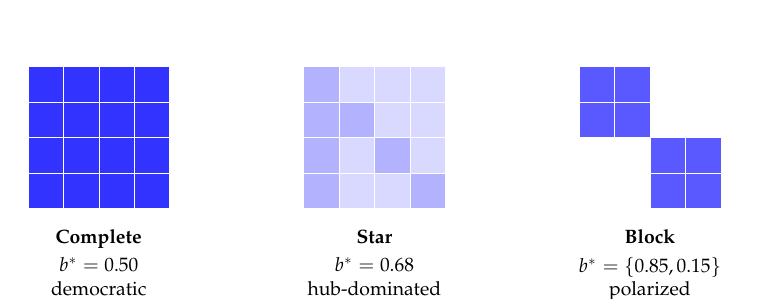
\begin{tikzpicture}[scale=1]
\def\N{4}
\def\s{0.45}

%% Complete
\foreach \i in {1,...,\N} {
  \foreach \j in {1,...,\N} {
    \fill[blue!80, draw=white, line width=0.15pt]
      ({(\j-1)*\s}, {(\N-\i)*\s}) rectangle +(\s,\s);
  }
}
\node[below, font=\scriptsize\bfseries] at ({2*\s}, -0.15) {Complete};
\node[below, font=\scriptsize] at ({2*\s}, -0.5) {$b^* = 0.50$};
\node[below, font=\scriptsize] at ({2*\s}, -0.8) {democratic};

%% Star
\begin{scope}[xshift=3.5cm]
\foreach \i in {1,...,\N} {
  \foreach \j in {1,...,\N} {
    \pgfmathparse{(\j==1) ? 75 : (\i==\j) ? 30 : 15}
    \edef\bp{\pgfmathresult}
    \fill[blue!\bp, draw=white, line width=0.15pt]
      ({(\j-1)*\s}, {(\N-\i)*\s}) rectangle +(\s,\s);
  }
}
\node[below, font=\scriptsize\bfseries] at ({2*\s}, -0.15) {Star};
\node[below, font=\scriptsize] at ({2*\s}, -0.5) {$b^* = 0.68$};
\node[below, font=\scriptsize] at ({2*\s}, -0.8) {hub-dominated};
\end{scope}

%% Block-diagonal
\begin{scope}[xshift=7cm]
\foreach \i in {1,...,\N} {
  \foreach \j in {1,...,\N} {
    \pgfmathparse{(\i<=2 && \j<=2) ? 65 : (\i>2 && \j>2) ? 65 : 0}
    \edef\bp{\pgfmathresult}
    \fill[blue!\bp, draw=white, line width=0.15pt]
      ({(\j-1)*\s}, {(\N-\i)*\s}) rectangle +(\s,\s);
  }
}
\node[below, font=\scriptsize\bfseries] at ({2*\s}, -0.15) {Block};
\node[below, font=\scriptsize] at ({2*\s}, -0.5) {$b^* = \{0.85, 0.15\}$};
\node[below, font=\scriptsize] at ({2*\s}, -0.8) {polarized};
\end{scope}
\end{tikzpicture}
\end{center}
\vspace{-0.5em}
\small Same initial beliefs (0.9, 0.8, 0.2, 0.1). Three different $W^I$'s produce three different outcomes: democratic consensus, hub-dominated consensus, and permanent polarization. The heatmap determines the epistemic outcome.
\end{vizpanel}


%% =====================================================================
\section{The Wisdom and Foolishness of Crowds}
\label{sec:wisdom}
%% =====================================================================

\subsection{Wisdom: When Does the Consensus Get It Right?}

\begin{theorem}[Wisdom of Crowds --- Golub and Jackson 2010]\label{thm:wisdom}
Suppose the true state is $\omega$, and agent $i$'s initial belief is $b_i^{(0)} = \omega + \varepsilon_i$, where $\varepsilon_i$ is a zero-mean noise with variance $\sigma_i^2$. The DeGroot consensus is:
\begin{equation}
b^* = \omega + \sum_j \pi^I_j \varepsilon_j.
\end{equation}
The consensus error is $e = b^* - \omega = \sum_j \pi^I_j \varepsilon_j$, with:
\begin{equation}\label{eq:wisdom}
\Var(e) = \sum_{j=1}^N (\pi^I_j)^2 \sigma_j^2 \geq \frac{\bar{\sigma}^2}{N_{\text{eff}}},
\end{equation}
where $N_{\text{eff}} = 1/\sum_j (\pi^I_j)^2$ is the \textbf{effective sample size}.
\end{theorem}

\begin{proof}
$\Var(e) = \Var(\sum_j \pi^I_j \varepsilon_j) = \sum_j (\pi^I_j)^2 \sigma_j^2$ (assuming independent errors). By Cauchy-Schwarz: $\sum_j (\pi^I_j)^2 \geq 1/N$ with equality iff $\pi^I_j = 1/N$ for all $j$.
\end{proof}

\begin{definition}[Effective Sample Size]\label{def:neff}
$N_{\text{eff}} = 1 / \sum_j (\pi^I_j)^2$. This is the number of ``independent voices'' in the consensus. When $\boldsymbol{\pi}^I = \frac{1}{N}\ones$: $N_{\text{eff}} = N$ (every agent counts equally). When $\boldsymbol{\pi}^I \approx e_1$ (star): $N_{\text{eff}} \approx 1$ (only the hub's signal matters). The Herfindahl index of epistemic power is $H = 1/N_{\text{eff}}$.
\end{definition}

\begin{intuition}[The crowd is wise when power is equal]
The wisdom-of-crowds effect requires many independent signals to be aggregated with equal weight. When $W^I$ concentrates epistemic power, the consensus overweights a few agents' signals and underweights the rest. The effective sample size shrinks. The consensus becomes less accurate, not because individuals are dumber but because the network throws away most of the available information.

In a society where 5\% of the population controls 90\% of the media, $N_{\text{eff}} \approx 0.05N$. The society is epistemically 20 times poorer than it needs to be.
\end{intuition}


\subsection{Foolishness: Misinformation in Asymmetric Networks}

\begin{proposition}[Misinformation Amplification]\label{prop:misinfo}
If the hub in a star network has a biased initial belief ($b_h^{(0)} = \omega + \delta$ for some bias $\delta \neq 0$), the consensus inherits the bias:
\begin{equation}
b^* = \omega + \pi^I_h \delta + \text{noise}.
\end{equation}
The bias in the consensus is proportional to $\pi^I_h$: the hub's epistemic power. When $\pi^I_h \to 1$, the consensus reproduces the hub's bias exactly.
\end{proposition}

This is the misinformation mechanism: a biased agent with high epistemic power contaminates the entire network. The contamination is permanent (it enters the long-run consensus) and is not self-correcting (DeGroot agents do not learn from prediction errors). The only correction is structural: change $W^I$ to reduce the hub's epistemic power.

\begin{prebisch}[The Washington Consensus as a DeGroot equilibrium]
The Washington Consensus of the 1990s --- fiscal discipline, trade liberalization, privatization, deregulation --- was not imposed by force on most countries. It was adopted because the information network $W^I_{\text{global}}$ had a hub-spoke topology: the IMF, World Bank, and US Treasury were the dominant nodes, and peripheral policymakers updated their beliefs by listening to these institutions.

In DeGroot terms: $\pi^I_{\text{IMF}} + \pi^I_{\text{WB}} + \pi^I_{\text{UST}} \approx 0.6$ (these three institutions controlled roughly 60\% of the global epistemic weight on economic policy). The consensus $b^*$ converged to their shared priors: markets work, governments fail, structural adjustment is necessary. The $N - 3$ other agents' priors (including the structuralists at CEPAL, who had different priors about the role of the state) had negligible weight in the consensus because their epistemic power $\pi^I_j$ was small.

The consensus was not wrong because markets never work. It was wrong because $N_{\text{eff}} \approx 3$ in a world with hundreds of relevant economies. The wisdom of the crowd was thrown away by the network topology.
\end{prebisch}


%% =====================================================================
\section{Belief Manipulation}
\label{sec:manipulation}
%% =====================================================================

\subsection{The Manipulation Problem}

Suppose a \textit{manipulator} --- a government, a media company, a foreign power --- wants to steer the consensus to a target belief $b_T$. She cannot change agents' initial beliefs directly, but she can change the information network $W^I$: by controlling media outlets, shaping algorithms, subsidizing certain voices, or silencing others.

\begin{definition}[Manipulation Cost]\label{def:manip_cost}
Given the current network $W^I$ with Perron eigenvector $\boldsymbol{\pi}^I$ and initial beliefs $\bb^{(0)}$, the current consensus is $b^* = (\boldsymbol{\pi}^I)'\bb^{(0)}$. The manipulator wants to achieve a target $b_T$. The \textbf{manipulation cost} is:
\begin{equation}\label{eq:manip_cost}
C(b_T) = \min_{\Delta W^I} \left\{\|\Delta W^I\|_F : (\boldsymbol{\pi}^I(W^I + \Delta W^I))'\bb^{(0)} = b_T\right\},
\end{equation}
subject to $W^I + \Delta W^I$ remaining row-stochastic and nonnegative.
\end{definition}

\begin{theorem}[Manipulation Theorem]\label{thm:manipulation}
For small perturbations ($\|\Delta W^I\|_F$ small):
\begin{equation}\label{eq:manip_result}
C(b_T) \propto \frac{|b_T - b^*|}{\max_j |b_j^{(0)} - b^*|} \cdot \frac{1}{\Gamma^I},
\end{equation}
where $\Gamma^I$ is the spectral gap of $W^I$.
\end{theorem}

\begin{intuition}[What makes manipulation cheap?]
The cost of manipulation is low when:

\textbf{(i) The target belief is close to the current consensus} ($|b_T - b^*|$ small). Nudging is cheap.

\textbf{(ii) Initial beliefs are diverse} ($\max_j |b_j - b^*|$ large). The manipulator can amplify an existing minority voice rather than creating a new one.

\textbf{(iii) The spectral gap is small} ($\Gamma^I \approx 0$). Small changes in the network produce large changes in $\boldsymbol{\pi}^I$ when the eigenvalues are close together. The consensus is structurally fragile.

The most manipulable society is one with a fragmented information network (small $\Gamma^I$), diverse initial beliefs, and a target close to an already-existing minority view. Echo chambers plus polarization plus a skilled manipulator: the conditions for epistemic capture.
\end{intuition}


\subsection{The Algorithmic Manipulator}

In the pre-digital era, manipulation required owning a newspaper or a radio station: physically controlling a hub in $W^I$. In the algorithmic era, manipulation operates through the \textit{edges} of $W^I$ rather than the nodes: the algorithm determines $W^I_{ij}$ (what content agent $i$ sees from agent $j$) for every pair simultaneously.

\begin{proposition}[Algorithmic Control of $W^I$]\label{prop:algorithm}
A platform that controls the recommendation algorithm chooses $W^I_{ij}$ for all $i, j$. This is equivalent to choosing $\boldsymbol{\pi}^I$ (and therefore $b^*$) directly, subject to the constraint that $W^I$ must be consistent with user engagement (agents must find the recommended content sufficiently interesting to consume).
\end{proposition}

\begin{example}[The Platform Economy]\label{ex:platform}
$N = 6$: three content creators (C1, C2, C3) and three consumers (U1, U2, U3). C1 produces pro-market content ($b_{C1} = 0.9$), C2 produces structuralist content ($b_{C2} = 0.3$), C3 produces entertainment ($b_{C3} = 0.5$).

\textbf{Organic $W^I$:} Each consumer follows all three creators equally: $W^I_{U_k, C_j} = 1/3$ for all $k, j$. Consensus: $b^* = (0.9 + 0.3 + 0.5)/3 = 0.567$.

\textbf{Algorithmic $W^I$:} The platform's engagement algorithm shows consumers content that confirms their priors. U1 (prior 0.8) sees mostly C1; U3 (prior 0.2) sees mostly C2; U2 sees C3. The effective $W^I$ becomes block-diagonal. No single consensus forms; instead, two echo chambers: $b^*_1 \approx 0.85$ and $b^*_2 \approx 0.25$.

The algorithm did not inject misinformation. It reshaped $W^I$ from complete to block-diagonal, replacing one consensus with two polarized ones. The spectral gap collapsed from 1.0 to $\approx 0$.
\end{example}


%% =====================================================================
\section{From Beliefs to Preferences: The Bridge to Part III}
\label{sec:bridge}
%% =====================================================================

Everything so far treats beliefs as a one-shot process: initial beliefs are updated once and converge. But beliefs about returns shape investment decisions, which produce outcomes, which become signals, which update beliefs. The loop is dynamic.

\begin{proposition}[The Belief-Action-Signal Loop]\label{prop:loop}
Consider a sequence of generations $t = 0, 1, 2, \ldots$. In generation $t$:
\begin{enumerate}
\item Agents form beliefs about returns: $\hat{r}_{i,t} = \sum_j W^I_{ij} r_{j,t-1}$ (DeGroot on observed returns).
\item Agents choose actions based on beliefs: $a_{i,t} = f(\hat{r}_{i,t}, \theta_{i,t})$ (investment, education, labor supply).
\item Actions produce outcomes: $r_{i,t} = g(a_{i,t}, \x_t)$ (realized returns, depending on the allocation).
\item Outcomes become the next generation's signals.
\end{enumerate}
The steady state satisfies: $\hat{r}_i = \sum_j W^I_{ij} g(f(\hat{r}_j, \theta_j), \x^*)$ --- a fixed point of the belief-action-signal map.
\end{proposition}

\begin{keyinsight}
When $W^I$ is block-diagonal, the belief-action-signal loop produces \textbf{two different steady states in the same economy}. Block~1 (modern sector) observes high returns, forms optimistic beliefs, invests heavily, achieves high returns --- confirming the beliefs. Block~2 (traditional sector) observes low returns, forms pessimistic beliefs, underinvests, achieves low returns --- confirming those beliefs too.

Both blocks are in equilibrium. Both have ``rational'' beliefs (their beliefs match the returns they observe). But the traditional sector's beliefs are only rational \textit{conditional on the traditional sector's $W^I$}. If the girl in Potos\'{i} could observe the modern sector's returns (if $W^I$ had cross-block entries), she would form different beliefs, make different investments, and achieve different outcomes.

\textit{The structure produces the beliefs that justify the structure.}

This is the formation mechanism: $W^I$ shapes beliefs, beliefs shape preferences (through $\theta$), preferences shape the allocation, and the allocation confirms the beliefs. Part~III (Chapters~9--12) develops this fully.
\end{keyinsight}


%% =====================================================================
\section{Summary}
\label{sec:summary}
%% =====================================================================

\begin{enumerate}
\item \textbf{DeGroot learning} on $W^I$ converges to a consensus $b^* = (\boldsymbol{\pi}^I)'\bb^{(0)}$: the Perron-weighted average of initial beliefs. Epistemic power $\pi^I_j$ determines each agent's influence on the long-run consensus.

\item The \textbf{effective sample size} $N_{\text{eff}} = 1/\sum_j (\pi^I_j)^2$ measures the epistemic richness of the consensus. Concentrated $\boldsymbol{\pi}^I$ (asymmetric $W^I$) wastes information: $N_{\text{eff}} \ll N$.

\item \textbf{Misinformation amplification:} a biased hub contaminates the consensus in proportion to $\pi^I_h$. The contamination is permanent under DeGroot dynamics.

\item \textbf{Manipulation cost} is proportional to $|b_T - b^*| / \Gamma^I$: small spectral gap makes manipulation cheap. Algorithmic platforms choose $W^I$ directly, collapsing the spectral gap by creating echo chambers.

\item The \textbf{belief-action-signal loop} connects epistemic power to economic outcomes: $W^I$ shapes beliefs, beliefs shape actions, actions produce returns, returns become signals. When $W^I$ is block-diagonal, the loop produces self-confirming pessimism in the powerless block.
\end{enumerate}


%% =====================================================================
\section{Exercises}
\label{sec:exercises}
%% =====================================================================

\begin{enumerate}[label=\textbf{8.\arabic*}, leftmargin=3em]

\item \textbf{DeGroot by hand.} For $W^I = \begin{pmatrix} 0.5 & 0.3 & 0.2 \\ 0.1 & 0.6 & 0.3 \\ 0.3 & 0.2 & 0.5 \end{pmatrix}$ and $\bb^{(0)} = (1.0, 0.0, 0.5)'$:
\begin{enumerate}
\item Compute $\bb^{(1)}$, $\bb^{(2)}$, $\bb^{(3)}$ by hand.
\item Compute $\boldsymbol{\pi}^I$ (use the method from Chapter~6 or software).
\item Verify that $\bb^{(t)} \to b^*\ones$ and check $b^* = (\boldsymbol{\pi}^I)'\bb^{(0)}$.
\item What is the half-life of disagreement? (Compute $|\lambda_2|$.)
\end{enumerate}

\item \textbf{Effective sample size.} For $N = 100$, compute $N_{\text{eff}}$ for:
\begin{enumerate}
\item $\boldsymbol{\pi}^I = \frac{1}{100}\ones$ (complete graph).
\item $\pi^I_1 = 0.5$, $\pi^I_j = 0.5/99$ for $j \geq 2$ (one dominant hub).
\item $\pi^I_1 = 0.9$, $\pi^I_j = 0.1/99$ for $j \geq 2$ (state media monopoly).
\item Plot $N_{\text{eff}}$ as a function of $\pi^I_1$ (with the rest distributed uniformly). At what $\pi^I_1$ does $N_{\text{eff}}$ drop below 10?
\end{enumerate}

\item \textbf{Manipulation cost.} Using the three-agent network from Exercise 8.1:
\begin{enumerate}
\item The current consensus is $b^*$. A manipulator wants $b_T = 0.8$. Compute the required shift in $\boldsymbol{\pi}^I$.
\item What is the cheapest edge to change? (Hint: which edge has the largest effect on $\boldsymbol{\pi}^I$ per unit of perturbation?)
\item How does the cost change if $\Gamma^I$ doubles? If it halves?
\end{enumerate}

\item \textbf{The algorithm as $W^I$ designer.} Consider $N = 8$: 4 liberals ($b^{(0)}_i = 0.8$) and 4 conservatives ($b^{(0)}_i = 0.2$).
\begin{enumerate}
\item Under $W^I = \frac{1}{8}\ones\ones'$: what is the consensus? What is $\Gamma^I$?
\item Under $W^I$ = block-diagonal (liberals talk only to liberals, conservatives only to conservatives): what are the two ``consensuses''? What is $\Gamma^I$?
\item An engagement-maximizing algorithm assigns $W^I_{ij} \propto \exp(-\beta|b_i^{(0)} - b_j^{(0)}|)$ (agents see content similar to their prior). Compute $W^I$ for $\beta = 0, 1, 5, 20$. Plot $\Gamma^I(\beta)$.
\item At what $\beta$ does the society split from one consensus into two?
\end{enumerate}

\item \textbf{Bolivia's epistemic structure.} Bolivia has three major media markets: La Paz (state media dominant), Santa Cruz (private media dominant), and Cochabamba (mixed). Model this as $N = 3$ blocks.
\begin{enumerate}
\item Construct plausible $W^I$ matrices for each block (who listens to whom within each city's media ecosystem).
\item Compute $\boldsymbol{\pi}^I$ for the national composite.
\item Under what initial beliefs $\bb^{(0)}$ about economic policy (e.g., nationalization vs.\ liberalization) does the consensus favor nationalization? Liberalization?
\item How much would it cost (in $\|\Delta W^I\|_F$) to shift the consensus from 0.6 (mild pro-nationalization) to 0.4 (mild pro-liberalization)?
\end{enumerate}

\item \textbf{The belief-action-signal loop.} In a two-sector economy (Modern, Traditional):
\begin{enumerate}
\item Returns are $r_M = 0.15$ and $r_T = 0.05$. Under $W^I_{\text{block}} = \text{diag}(W_{11}, W_{22})$ (each sector observes only its own returns): what beliefs form in each sector?
\item An agent in the Traditional sector receives a smartphone (a new edge in $W^I$ connecting her to the Modern sector). Her belief about the return to education changes from $\hat{r} = 0.05$ to $\hat{r}' = 0.5 \times 0.05 + 0.5 \times 0.15 = 0.10$. If investment is $a = \theta \cdot \hat{r}$, by how much does her investment increase?
\item If 10\% of Traditional-sector agents receive smartphones, what is the effect on the sector's average belief? On $\Gamma^I$?
\item This is the formation mechanism of Part~III. Write down the full loop: $W^I \to \hat{r} \to a \to r \to$ (next period's signal). Under what condition is the Traditional sector's low-return equilibrium stable?
\end{enumerate}

\item \textbf{Quijano in matrix form.} Quijano (2000) argued that the ``coloniality of power'' operates through racial classification that structures all domains of social existence. Formalize:
\begin{enumerate}
\item Define $W^I$ where the epistemic weights correlate with racial classification: European-descended agents have $\pi^I_j \gg 1/N$; Indigenous agents have $\pi^I_j \ll 1/N$.
\item What consensus forms about the ``value'' of different forms of knowledge (Western science vs.\ traditional medicine, formal education vs.\ artisanal skill)?
\item How does this consensus shape preferences ($\theta$) regarding education, language, and economic aspiration?
\item What structural change in $W^I$ would Quijano's ``decoloniality'' require? Write it as a matrix perturbation.
\end{enumerate}
\end{enumerate}


%% =====================================================================
\newpage
\section*{Mathematical Appendices}
\addcontentsline{toc}{section}{Mathematical Appendices}
%% =====================================================================


\subsection*{Appendix 8A: Power Iteration and Convergence of $(W^I)^t$}
\addcontentsline{toc}{subsection}{Appendix 8A: Power Iteration}
\label{app:power_iteration}

\paragraph{Power iteration.} To compute the left Perron eigenvector $\boldsymbol{\pi}^I$:
\begin{enumerate}
\item Start with any initial vector $\boldsymbol{\pi}^{(0)} > 0$ with $\sum_i \pi^{(0)}_i = 1$.
\item Iterate: $\boldsymbol{\pi}^{(t+1)\prime} = \boldsymbol{\pi}^{(t)\prime} W^I$, then normalize $\boldsymbol{\pi}^{(t+1)} \leftarrow \boldsymbol{\pi}^{(t+1)} / \|\boldsymbol{\pi}^{(t+1)}\|_1$.
\item Convergence: $\|\boldsymbol{\pi}^{(t)} - \boldsymbol{\pi}^I\| \leq C |\lambda_2/\lambda_1|^t$.
\end{enumerate}

The convergence rate is $|\lambda_2/\lambda_1| = |\lambda_2|$ (since $\lambda_1 = 1$ for row-stochastic matrices). Large spectral gap = fast convergence.

\paragraph{Python implementation.}
\begin{verbatim}
import numpy as np

def perron_left(W, tol=1e-12, max_iter=10000):
    """Left Perron eigenvector of row-stochastic W."""
    n = W.shape[0]
    pi = np.ones(n) / n
    for _ in range(max_iter):
        pi_new = pi @ W
        pi_new /= pi_new.sum()
        if np.max(np.abs(pi_new - pi)) < tol:
            return pi_new
        pi = pi_new
    return pi
\end{verbatim}

\paragraph{Convergence of $(W^I)^t$.} Theorem~\ref{thm:degroot} states $(W^I)^t \to \ones(\boldsymbol{\pi}^I)'$. The rate: $\|(W^I)^t - \ones(\boldsymbol{\pi}^I)'\| \leq C |\lambda_2|^t$, where $C$ depends on the condition number of the eigenvector matrix.

For practical purposes: if $|\lambda_2| = 0.7$, then after $t = 10$ rounds, the error is $0.7^{10} \approx 0.028$ (2.8\%). After $t = 20$: $0.7^{20} \approx 0.0008$ (0.08\%). Consensus is essentially reached in $\approx 3/\Gamma^I$ rounds.


\subsection*{Appendix 8B: Sensitivity of $\boldsymbol{\pi}^I$ to Perturbations of $W^I$}
\addcontentsline{toc}{subsection}{Appendix 8B: Sensitivity Analysis}
\label{app:sensitivity}

\paragraph{The question.} If we perturb $W^I$ by a small $\Delta W^I$, how much does $\boldsymbol{\pi}^I$ change?

\paragraph{First-order perturbation.} Let $W^I$ have eigendecomposition with right eigenvectors $\mathbf{v}_k$ and left eigenvectors $\mathbf{u}_k$ (normalized so $\mathbf{u}_k'\mathbf{v}_k = 1$). The Perron eigenvector sensitivity:
\begin{equation}
\Delta\boldsymbol{\pi}^I \approx \sum_{k=2}^N \frac{1}{1 - \lambda_k} \mathbf{u}_k (\mathbf{u}_k' \Delta W^I \mathbf{v}_1) + O(\|\Delta W^I\|^2).
\end{equation}

The sensitivity is inversely proportional to $(1 - \lambda_k)$ for each eigenvalue. When $\lambda_2 \approx 1$ (small spectral gap), the sensitivity diverges: small perturbations in $W^I$ produce large changes in $\boldsymbol{\pi}^I$. This is why manipulation is cheap when $\Gamma^I$ is small.

\paragraph{Implication for manipulation.} The cheapest manipulation targets the eigenvector direction corresponding to $\lambda_2$ --- the direction of maximum sensitivity. In a block-diagonal $W^I$, this direction corresponds to the between-block balance: a small rewiring that shifts attention from one block to another produces a large shift in epistemic power.


%% =====================================================================
\subsection*{Structuralist Case Study: Quijano's Coloniality and the Epistemic Perron Vector}
\addcontentsline{toc}{subsection}{Structuralist Case Study: Quijano (2000)}
%% =====================================================================

An\'{i}bal Quijano (1930--2018) was a Peruvian sociologist whose 2000 essay ``Colonialidad del poder, eurocentrismo y Am\'{e}rica Latina'' (published in Lander, ed., \textit{La colonialidad del saber}) launched the decolonial turn in Latin American social theory. His argument was not about colonialism as a historical event but about \textbf{coloniality} as a persistent structure of power --- a structure that survived independence and continues to organize knowledge, labor, and social classification in the postcolonial world.

Quijano's framework maps onto the three-network model of this book in a specific and illuminating way.

\textbf{Part 1: Racial classification as a node attribute that constrains $W$.} Quijano argued that the colonial invention of ``race'' was not a byproduct of conquest but its \textit{organizing principle}: a classification system that assigned social position on the basis of phenotype. In network terms: race is a \textbf{node attribute} that determines which edges exist in $W^U$, $W^P$, and $W^I$ simultaneously. People of European descent form dense connections among themselves across all three networks; people classified as ``Indian'' or ``Black'' are confined to sparse, peripheral positions. The weight matrix is not random or purely economic --- it is structured by a categorical attribute that was imposed by conquest and maintained by institutional inertia.

\textbf{Part 2: Epistemic coloniality is $\boldsymbol{\pi}^I$ dominance.} The deepest dimension of coloniality, for Quijano, is epistemic: the colonial powers did not merely control trade routes and labor --- they controlled the \textit{definition of knowledge}. European science, philosophy, and social theory were installed as the universal standard; all other forms of knowledge were classified as ``traditional,'' ``local,'' ``pre-modern.'' In this chapter's notation: the global $W^I$ assigns European intellectual traditions a Perron weight $\pi^I_{\text{Euro}} \gg 1/N$, while Andean, African, and Asian intellectual traditions receive $\pi^I \approx 0$. The DeGroot consensus on ``what counts as knowledge'' converges to the European prior, not because that prior is more accurate but because $W^I$ is hub-dominated. The effective sample size is $N_{\text{eff}} \approx 1$ for epistemology: only one tradition's knowledge enters the consensus.

\textbf{Part 3: The coloniality of power operates across all three networks simultaneously.} Quijano's distinctive contribution was insisting that race structures $W^U$ (who you care about), $W^P$ (who you trade with and work for), and $W^I$ (whose knowledge you accept) \textit{simultaneously and correlatively}. The Perron eigenvector rankings are \textit{aligned across networks}: the agents who are powerful in $W^U$ are also powerful in $W^P$ and in $W^I$, and this alignment is not a coincidence but a structural feature maintained by the racial classification system. In the notation of Chapter~5: the three networks satisfy $\boldsymbol{\pi}^U \approx \boldsymbol{\pi}^P \approx \boldsymbol{\pi}^I$ --- the ``aligned networks'' case, which produces the maximum possible power concentration in the composite.

\begin{center}
\begin{tabular}{lll}
\toprule
\textbf{Quijano's argument} & \textbf{Formal object} & \textbf{This chapter} \\
\midrule
Race as organizing principle & Node attribute constraining $W$ & All three networks \\
Epistemic coloniality & $\pi^I_{\text{Euro}} \gg 1/N$ & Def.~\ref{def:epistemic_power} \\
One tradition dominates & $N_{\text{eff}} \approx 1$ & Def.~\ref{def:neff} \\
Consensus reproduces colonial priors & $b^* \approx b_{\text{Euro}}$ & Thm.~\ref{thm:degroot} \\
Power aligned across networks & $\boldsymbol{\pi}^U \approx \boldsymbol{\pi}^P \approx \boldsymbol{\pi}^I$ & Ch.~5, aligned case \\
Decoloniality as structural change & Rewire $W^I$ to equalize $\boldsymbol{\pi}^I$ & Thm.~\ref{thm:manipulation} \\
\bottomrule
\end{tabular}
\end{center}

Quijano's decolonial project is, in matrix terms, a call to \textit{rewire $W^I$ so that $\boldsymbol{\pi}^I$ equalizes across racial categories}. This does not mean all knowledge traditions are equally accurate (that is an empirical question). It means all traditions should have equal \textit{voice} in the DeGroot process --- equal epistemic power --- so that the consensus reflects $N_{\text{eff}} = N$ rather than $N_{\text{eff}} = 1$. The wisdom-of-crowds theorem (Theorem~\ref{thm:wisdom}) tells us that this equalization would make the consensus more accurate, not less, as long as different traditions carry independent information.

Quijano wrote in Spanish, from Lima. He did not have the Perron eigenvector. He had the diagnosis: that the pattern of power is maintained not primarily by guns but by the control of what counts as knowledge. This chapter gives that diagnosis its eigenvalue.


%% =====================================================================
\subsection*{Further Reading}
\addcontentsline{toc}{subsection}{Further Reading}
%% =====================================================================

\textbf{DeGroot learning:} DeGroot (1974), ``Reaching a Consensus,'' \textit{JASA}. Golub and Jackson (2010), ``Na\"{i}ve Learning in Social Networks and the Wisdom of Crowds,'' \textit{AEJ: Microeconomics} --- the key paper, proving the wisdom-of-crowds result and the effective sample size formula.

\textbf{Bayesian vs.\ na\"{i}ve learning:} Acemoglu, Dahleh, Lobel, and Ozdaglar (2011), ``Bayesian Learning in Social Networks,'' \textit{ReStud}. Jadbabaie, Molavi, Sandroni, and Tahbaz-Salehi (2012), ``Non-Bayesian Social Learning,'' \textit{Games and Economic Behavior}.

\textbf{Misinformation and manipulation:} Acemoglu, Ozdaglar, and ParandehGheibi (2010), ``Spread of (Mis)information in Social Networks,'' \textit{Games and Economic Behavior}. Candogan and Drakopoulos (2020), ``Optimal Signaling of Content Accuracy.'' Allcott and Gentzkow (2017), ``Social Media and Fake News in the 2016 Election,'' \textit{JEP}.

\textbf{Decolonial theory:} Quijano (2000), ``Colonialidad del poder, eurocentrismo y Am\'{e}rica Latina,'' in Lander (ed.), \textit{La colonialidad del saber}, Buenos Aires: CLACSO (the primary source). Mignolo (2000), \textit{Local Histories/Global Designs}. For the connection to economics: Ndikumana and Boyce (2011), \textit{Africa's Odious Debts}, Chapter~1.

\textbf{Algorithmic information networks:} Ribeiro et al.\ (2020), ``Auditing Radicalization Pathways on YouTube.'' Huszar et al.\ (2022), ``Algorithmic Amplification of Politics on Twitter,'' \textit{PNAS}.


\end{document}
